\documentclass{article}

% use Times
\usepackage{times}
% For figures
\usepackage{graphicx} % more modern
\usepackage{subfigure} 

% For citations
\usepackage{natbib}

% For algorithms
\usepackage{algorithm}
\usepackage{algorithmic}

% For hyperlinks
\usepackage{hyperref}

% Packages hyperref and algorithmic misbehave sometimes.  We can fix
% this with the following command.
\newcommand{\theHalgorithm}{\arabic{algorithm}}

\usepackage[accepted]{icml2015}


% The \icmltitle you define below is probably too long as a header.
% Therefore, a short form for the running title is supplied here:
\icmltitlerunning{Parallel Backpropagation for Multilayer Neural Networks}

\begin{document} 

\twocolumn[
\icmltitle{Parallel Backpropagation for Multilayer Neural Networks}

% It is OKAY to include author information, even for blind
% submissions: the style file will automatically remove it for you
% unless you've provided the [accepted] option to the icml2015
% package.
\icmlauthor{Nitin Kamra}{nkamra@usc.edu}
\icmladdress{Department of Computer Science, University of Southern California}
\icmlauthor{Palash Goyal}{palashgo@usc.edu}
\icmladdress{Department of Computer Science, University of Southern California}
\icmlauthor{Sungyong Seo}{sungyons@usc.edu}
\icmladdress{Department of Computer Science, University of Southern California}
\icmlauthor{Vasileios Zois}{vzois@usc.edu}
\icmladdress{Department of Computer Science, University of Southern California}

% You may provide any keywords that you 
% find helpful for describing your paper; these are used to populate 
% the "keywords" metadata in the PDF but will not be shown in the document
\icmlkeywords{machine learning, neural network, backpropagation, gradient descent, parallel backpropagation}

\vskip 0.3in
]

\begin{abstract} 
\end{abstract} 

\section{Introduction}
\label{Intro}

Artificial neural networks are powerful machine learning tools used in many applications including but not limited to search engines, spam and fraud detection, image classification, diagnostic medicine applications and stock market prediction.

Prior to application, neural networks undergo a training phase which is known to be very computationally intensive. This is primarily because the prevailing neural network architectures are implemented using several hidden layers, with each one consisting of thousands to millions of neurons in order to generalize well on diverse inputs. In this case, the resulting number of parameters that need to be trained are in the order of millions.

Furthermore, achieving high accuracy requires considering a large number of training examples (usually in the order of millions). For this reason training a neural network is both a data and resource intensive operation. This calls for efforts to parallelize the training process on multi-core and while emphasizing at utilizing the maximum available bandwidth.

Currently Minibatch Gradient Descent (henceforth called MGD) is the most commonly used optimization algorithm used to train neural networks in supervised settings. It is implemented in a layerwise-recursive fashion which is termed \textit{backpropagation} in the context of neural networks.

In this paper, we have implemented parallel backpropagation to train Multi Layer Perceptrons (MLPs) for classification tasks.
The rest of the paper is organized as follows: section \ref{ProbDesc} presents a description of supervised learning tasks and neural networks as classifiers. Section \ref{BackProp} describes the conventional serial backpropagation algorithm, and an approach to parallelization using multiple threads. Section \ref{GPUBackProp} describes how to implement backpropagation on a GPU with cuda. Section \ref{Exp} describes our datasets and the experiments we performed on them. Section \ref{Results} presents our results obtained for these implementations and analyzes the speedup obtained for various network architectures and increasing problem sizes. It also presents a comparison with the same algorithms implemented using a state-of-the-art neural network library Theano. Finally, we conclude in section \ref{Future} with a discussion of potential applications and future work for this project.

\section{Problem Description}
\label{ProbDesc}

We first formally describe a classification task in the supervised learning setting. Then we describe a feedforward neural network with fully connected layers. Feedforward neural networks act as function approximators in such tasks.

\subsection{Classification Problem}
\label{sub:ClassProb}

More formally, given a dataset $\mathcal{D} = \{x^{(i)},y^{(i)}\}_{i=1:N}$ with data points $x^{(i)} \in \mathbb{R}^D$ and labels $y^{(i)} \in \mathbb{R}^P$, the classification task involves making an accurate label prediction $\hat{y}$ on a previously unseen data point $x$. We approximate the label as a function of the datapoint using a classifier (a feedforward neural network here) with parameters $\theta = \{\theta_k\}_{k=1:K}$ as follows: $y \approx \hat{y} = f(x; \theta)$.
The classifier (neural network) learns the function $f$ from the training data $\mathcal{D}$ by tuning its parameters ($\theta$) to minimize a pre-specified loss function, for instance, the Mean-Squared Error loss:
\begin{align} \label{LMSE}
\mathcal{L}_{MSE} (\theta) = \frac{1}{N}\sum_{i=1}^N ( y^{(i)} - f(x^{(i)}; \theta))^2
\end{align}

This minimization can be carried out using optimization algorithms like Gradient Descent, Newton's method, Levenberg-Marquardt algorithm etc.
Though Newton's method is a second-order optimization technique, it requires the computation of the hessian of the objective function which is very prohibitive for a large number of parameters like in a neural network.
Levenberg-Marquardt algorithm also requires computing matrices of the size of hessian and can be very slow for classifiers with a large number of parameters.
Currently Gradient Descent is the most successful technique to train huge neural networks with millions of parameters, since it provides a decent tradeoff between convergence speed and memory requirements.
We will describe gradient descent in section \ref{GD}.

\subsection{Feedforward Neural Networks}
\label{sub:FNN}

\begin{figure}[ht]
%\vskip 0.2in
\begin{center}
\centerline{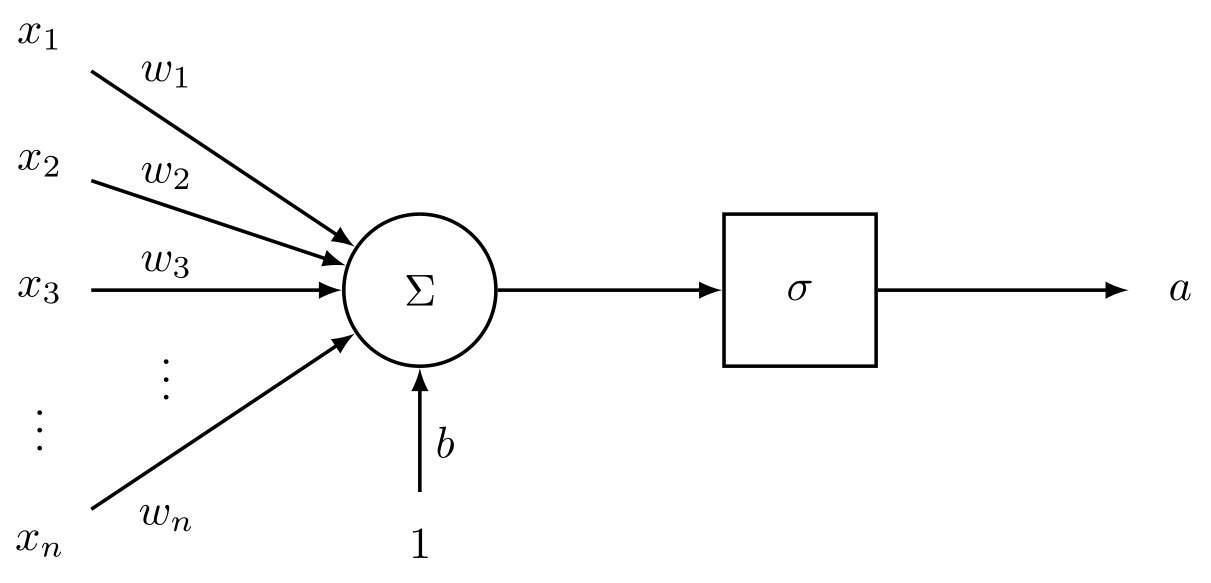
\includegraphics[width=\columnwidth]{neuron.png}}
\caption{A neuron}
\label{fig:neuron}
\end{center}
\vskip -0.2in
\end{figure}

The basic unit of feedforward neural networks is a neuron (figure \ref{fig:neuron}). A single neuron generally takes a vector of inputs $x \in \mathbb{R}^n$ and outputs a single scalar $a \in \mathbb{R}$ (called its activation). Generally the function computed by a neuron comprises of linear transformation on the input vector followed by a pointwise non-linear activation function:
\begin{align}
a = f(w^T x + b)
\end{align}
where $w \in \mathbb{R}^n$ is called the weight vector and $b \in \mathbb{R}$ is the scalar bias of the neuron.
Many different kinds of activation functions have been studied and used according to the task at hand e.g. linear, sigmoid, tanh, ReLU etc. We will use the sigmoid and linear$(f(z) = z)$ activation functions in our implementation.

\begin{figure}[ht]
%\vskip 0.2in
\begin{center}
\centerline{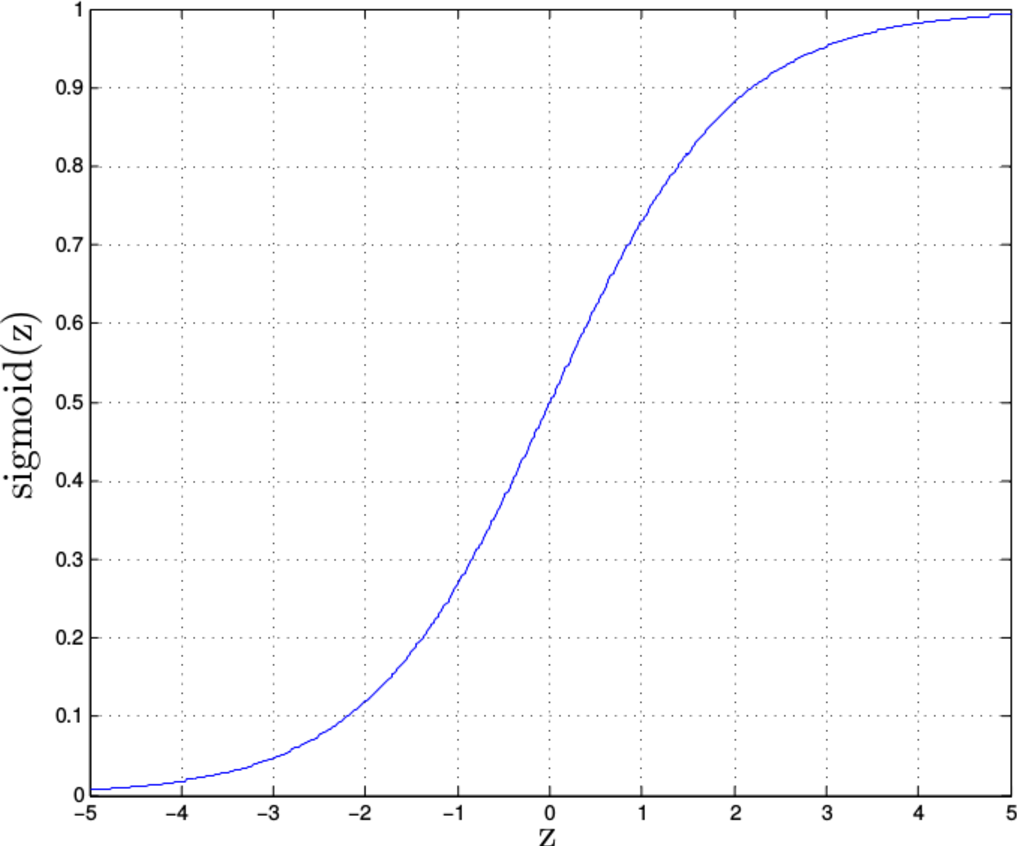
\includegraphics[width=0.7\columnwidth]{sigmoid.pdf}}
\caption{The sigmoid function}
\label{fig:sigmoid}
\end{center}
\vskip -0.2in
\end{figure}

The sigmoid function is shown in figure \ref{fig:sigmoid} and is defined as follows:
\begin{align}
\sigma(z) = \frac{1}{1 + e^{-z}}
\end{align}
A feedforward neural network is a directed acyclic graph $G = (V,E)$ each of whose vertices $v \in V$ is a neuron and every edge $(u,v) \in E$ represents the output of neuron $u$ going as an input to neuron $v$. In general to have a more concrete structure the graph $G$ is organized into a layered structure and we will only use layered feedforward neural networks in our implementations. 

A feedforward network with $L$ layers comprises of a single input layer, $L-2$ hidden layers (their outputs are not directly observed) and a final output layer.
Let the input of the neural network be $x \in \mathbb{R}^{n_{in}}$ and the output be $y \in \mathbb{R}^{n_{out}}$.
The $l^{th}$ layer has $n_l$ neurons and the full network has $n = \sum_{l=1}^L n_l$ neurons. 
An example network is shown in figure \ref{fig:nnet}.

\begin{figure}[ht]
%\vskip 0.2in
\begin{center}
\centerline{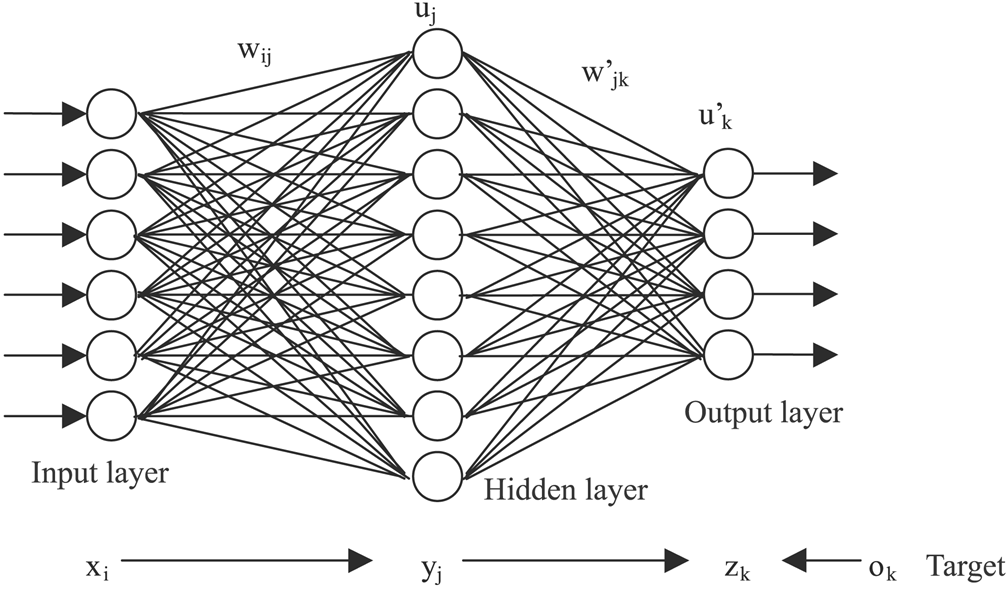
\includegraphics[width=\columnwidth]{nnet.png}}
\caption{A neural network with one hidden layer}
\label{fig:nnet}
\end{center}
\vskip -0.2in
\end{figure}

The input to the first layer (denoted $x_1$) is $x$ and the output (activation) of the first layer is denoted $a_1 \in \mathbb{R}^{n_{in}}$. The input layer contains $n_1 = n_{in}$ dummy neurons each of which takes a single scalar input $n_{in}$ and passes it as it is i.e. $a_1 = x_1 = x$.

All subsequent layers $l \in \{2,3,...,L\}$ give an output $a_l \in \mathbb{R}^{n_{l}}$ and take an input $x_l = a_{l-1} \in \mathbb{R}^{n_{l-1}}$. The final network output $y$ is given by $a_L \in \mathbb{R}^{n_L} (n_L = n_{out})$.
Each of these layers applies a linear transformation to its input followed by a pointwise non-linear activation function i.e. for each layer:
\begin{align}
z_l &= (W_l)^T x_l + b_l \\
a_l &= f(z_l)
\end{align}
where $W^l \in \mathbb{R}^{n_{l-1} \times n_l}$ is the weight matrix of the layer and $b_l \in \mathbb{R}^{n_l}$ is the bias vector. The function $f(\cdot)$ is the pointwise activation function which applies to each component of the $z_l$ vector and we will use sigmoid as our activation function for the classification task.


\section{Serial and Parallel Backpropagation}
\label{BackProp}

Describe backpropagation serial implementation in detail

Describe platform used \\
Describe backpropagation parallelization using pthreads


\section{Parallel Multicore Backpropagation}
\label{ParBackProp}

Describe platform used \\
Describe backpropagation parallelization using pthreads


\section{Parallel GPU Backpropagation}
\label{GPUBackProp}

Describe platform \\
Describe CUDA implementation for GPU

\section{Experimental setup}
\label{Exp}
In this section, we first describe the datasets used for our experiments and the corresponding classification tasks. We then delineate the networks used for each of these datasets and the procedure to determine the values of hyperparameters. This is followed by a description of the evaluation metric of the speedup. All the algorithms were implemented in C++. The reported results were obtained on a Ubuntu 14.04.4 LTS system with 32 cores, 128 GB RAM and a clock speed of 2.6 GHz.  

\subsection{Dataset description}
\label{sub:data_desc}
We test the speedups achieved by the parallel implementation on two public datasets - MNIST and KDD Cup 1999. These datasets have been widely used by the machine learning community to compare different learning algorithms. Their description is as follows:

\begin{itemize}
\item \textbf{MNIST} - This is an image database of handwritten digits which is commonly used for training various image processing systems (Figure \ref{fig:mnist}). The task here is to classify the digit in the image. This dataset was derived from NIST's datasets and was formed by mixing the samples from NIST. This mixing was done because the training and testing datasets in the original NIST dataset were obtained from two different groups of people (Census Bureau employees and high school students). This dataset consists of 60,000 training images and 10,000 testing images, each of size 28$\times$ 28. In our experiments, we further divided the training set into training and validation in 5:1 ratio in order to determine suitable values for the hyperparameters.

\begin{figure}
  \centering
       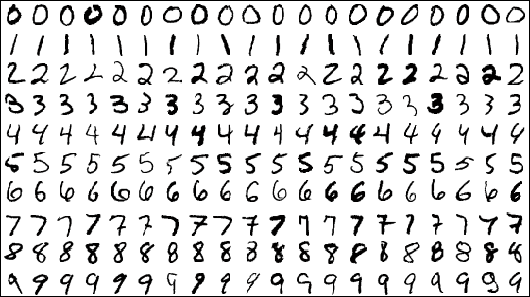
\includegraphics[scale=0.43]{mnist.png}
  \caption{MNIST dataset}
  \label{fig:mnist}
\end{figure}

\item \textbf{KDD Cup 1999} -  This is a dataset which first appeared in the KDD Cup held in 1999. The dataset has about 4 million data points each of which has 42 features. The features are of two types - categorical and integer. The task in the competition was to build a network intrusion detector which can be used to distinguish between good and bad network connections. 
\end{itemize}

\subsection{Network details}
\label{sub:net_det}
We now describe the details of the structure of neural networks used. For our experiments, we use two different configurations of neural network - 
\begin{itemize}
\item \textbf{Net-1h} - This network consists of 3 layers - input layer, one hidden layer and output layer. The input layer has 784 neurons for MNIST dataset and 42 neurons for KDD Cup 1999. The hidden layer is composed of 1024 neurons and the output layer has 10 neurons when used for MNIST dataset and 1 output for KDD Cup 1999.
\item \textbf{Net-2h} - This network is composed of 4 layers - input layer, two hidden layers and output layer. The input and output layer are same as Net-1h and each of the hidden layers has 1024 neurons.
\end{itemize}

\subsection{Hyperparameter selection}
\label{sub:hyper_sel}
Hyperparameter selection, also known as model selection, is an important problem in machine learning. It refers to choosing the optimal hyperparameters for a learning algorithm. It is crucial to select the values for hyperparameters which generalize well. This enables the algorithm to perform well on test data.

In the context of neural networks, hyperparameters refer to learning rate and regularization constant. Since our implementation is free of regularization, we only have one hyperparameter - learning rate. To choose an optimal learning rate, we used the technique of grid search. As mentioned above, we divide the training set into training and validation. We use different learning rates defined in a grid and test the accuracy on the validation data. The rate which gives the highest accuracy on validation is chosen and used to evaluate the performance of the algorithm on test data.

\subsection{Evaluation methodology}
\label{sub:eval}
As has been previously mentioned, this work aims to speed up the learning of neural network by parallelizing backpropagation and running it on GPU. To evaluate our approach and quantify the usefulness of parallelization, we use speed up as our primary measure. We calculate this with respect to the serial implementation on the same network configuration. Speed up may sometimes be misleading and does not capture the efficiency of serial implementation. To resolve this we use another measure - GFLOPS (Billion Floating Point Operations Per Second). This measure is independent of serial implementation and can be used to supplement the speedup metric.

\subsection{Experiments}
\label{sub:exp}
In this paper, we implement the gradient descent algorithm for training neural network. The implementation is 3-fold - serial, parallelization with Pthreads and parallelization with CUDA. The implementation follows from section \ref{BackProp} and section \ref{GPUBackProp}. Please refer to these sections for a detailed explanation of the methods.




\section{Results and Analysis}
\label{Results}

%Provide experiment results: serial \\
%Compare serial vs pthreads vs cuda vs theano. \\
%Provide graphs for speedup with increasing problem size \\
%Analyze speedup with number of threads/cores used \\
%Analyze the level of parallelization obtained \\
%Analyze performance bottlenecks \\
%Do overall analysis and compare obtained results with your expectations\\

As described in previous sections, we compare our implementations with state of the art deep learning library, Theano, in three different parallelizations (Serial/Pthreads/Cuda-C). All experiments are done under the same network structures with MNIST datasets and the number of threads is fixed as 32.

\begin{figure}[ht]
%\vskip 0.2in
\begin{center}
\centerline{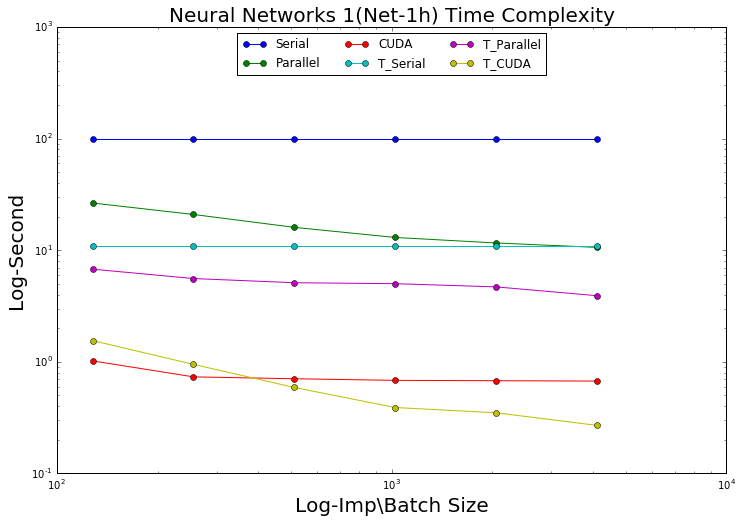
\includegraphics[width=\columnwidth]{../../slide/nn1_time.png}}
\caption{Learning time for Net-1h}
\label{fig:nn1_time}
\end{center}
\vskip -0.4in
\end{figure}

Figure \ref{fig:nn1_time} clearly shows distinct characteristics between serial and parallel computation as well as CPU and GPU based computation. First, the training time for 1 epoch of the serial implementation (Blue curve and Light blue curve) is almost constant over the varying mini batch size. It is obvious result because regardless of the size of each mini batch training data is accessed sequentially. On the other hand, the parallel learning time (Green curve) shows decreased training time due to multithreads distribution as we expected. One thing we should note is that the parallelism is enhanced when larger size of batch is used because the number of allocations of data into each thread is reduced. When smaller batch size is used, we need to assign each data into the corresponding thread more frequently and it causes more overheads. Moreover, as the last step, we need to combine all the results from every threads (which is called the reduction process) and the number of the reduction processes is also increased for smaller batch size. This behavior is shown commonly in the parallel computation based on Theano (T-Parallel).\\
In case of GPU based computation, the overall performance is significantly improved because GPU usually have much more cores which are specialized for repetitive operations such as matrix multiplications than CPU. As a result, GPU provides much faster learning time than that of CPU in general due to less number of allocation/reduction processes.\\
The faster computation by the parallelization is able to be captured by calculating GFLOPS. Figure \ref{fig:nn1_gflops} shows that parallelization provide much larger number of floating point operations than serial, thus, single thread computation.
\begin{figure}[ht]
%\vskip 0.2in
\begin{center}
\centerline{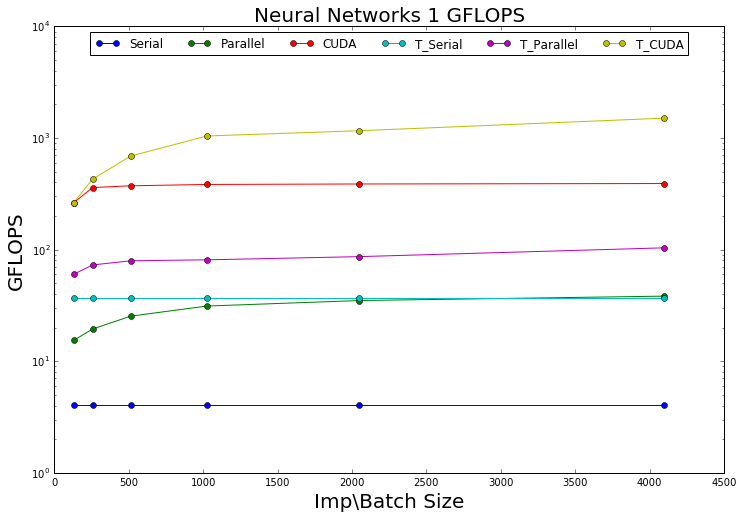
\includegraphics[width=\columnwidth]{../../slide/nn1_gflops.png}}
\caption{GFLOPS for Net-1h}
\label{fig:nn1_gflops}
\end{center}
\vskip -0.4in
\end{figure}

\textbf{BLAS} As Basic Linear Algebra Subprograms, BLAS has been crucial workhorse in heavy numerical computing. By replacing the self-built matrix-vector product libraries with BLAS functions, we could obtain hugely improved results (even faster than Theano). Note that the execution time of BLAS doesn't depend on the number of threads because it parallelizes each Matrix-vector product and hence each thread executes different parts of the same example. The serial implementation is still a bit slower than Theano but is faster than our previous implementation by about 10 times. This way shows that the optimized parallelism gives speed-up over Naive serial implementation. \\

\textbf{Bottleneck} In ideal case, by increasing the size of the batch, the number of overheads (allocation/reduction) is exponentially decreased. However, our experiment results show that there are some performance bottlenecks. In our implementation, shared memory bank conflicts which reduce the parallelism when threads access the shared memory appear when the number of batch increases. When the dimensions (i.e.number of neurons between layers) of the neural network is not perfect multiple of 32 then some threads do not participate in the computation so they are doing no work but still have to wait on the barrier. As a result, it causes degraded parallelism.\\

Overall, we demonstrate that the parallel computation is significantly faster than the serial computation by utilizing multithreads based on the mini batch in the multicore machine. Moreover, by dividing training datasets into larger mini batches, we are able to better performance than that of smaller batch size due to reduced overheads. Similarly, the training time and GFLOPS are improved in the second networks (Net-2h) (See Figure \ref{fig:nn2_time},\ref{fig:nn2_gflops}). 
\begin{figure}[ht]
%\vskip 0.2in
\begin{center}
\centerline{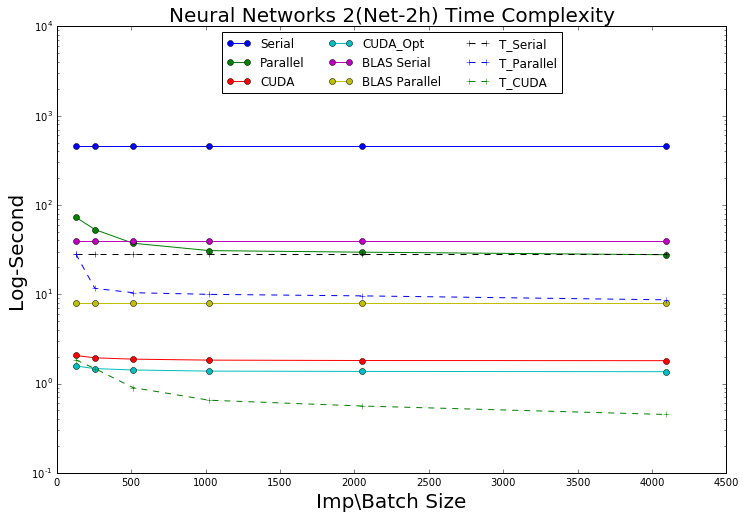
\includegraphics[width=\columnwidth]{../../slide/nn2_time.png}}
\caption{Learning time for Net-2h}
\label{fig:nn2_time}
\end{center}
\vskip -0.4in
\end{figure}
\begin{figure}[ht]
\vskip 0.2in
\begin{center}
\centerline{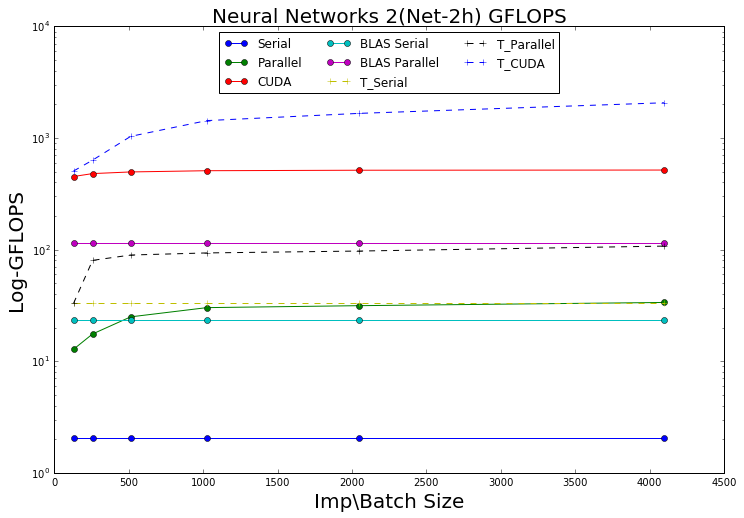
\includegraphics[width=\columnwidth]{../../slide/nn2_gflops.png}}
\caption{GFLOPS for Net-2h}
\label{fig:nn2_gflops}
\end{center}
\vskip -0.4in
\end{figure}





\section{Future Work}
\label{Future}

Discuss application of parallel training and future usage of this work

\bibliography{bibliography}
\bibliographystyle{icml2015}

\end{document} 

%\subsection{Figures}
%
%\begin{figure}[ht]
%\vskip 0.2in
%\begin{center}
%\centerline{\includegraphics[width=\columnwidth]{}}
%\caption{Historical locations and number of accepted papers for International
%  Machine Learning Conferences (ICML 1993 -- ICML 2008) and
%  International Workshops on Machine Learning (ML 1988 -- ML
%  1992). At the time this figure was produced, the number of
%  accepted papers for ICML 2008 was unknown and instead estimated.}
%\label{icml-historical}
%\end{center}
%\vskip -0.2in
%\end{figure} 
%
%\subsection{Algorithms}
%
%If you are using \LaTeX, please use the ``algorithm'' and ``algorithmic'' 
%environments to format pseudocode. These require 
%the corresponding stylefiles, algorithm.sty and 
%algorithmic.sty, which are supplied with this package. 
%Algorithm~\ref{alg:example} shows an example. 
%
%\begin{algorithm}[tb]
%   \caption{Bubble Sort}
%   \label{alg:example}
%\begin{algorithmic}
%   \STATE {\bfseries Input:} data $x_i$, size $m$
%   \REPEAT
%   \STATE Initialize $noChange = true$.
%   \FOR{$i=1$ {\bfseries to} $m-1$}
%   \IF{$x_i > x_{i+1}$} 
%   \STATE Swap $x_i$ and $x_{i+1}$
%   \STATE $noChange = false$
%   \ENDIF
%   \ENDFOR
%   \UNTIL{$noChange$ is $true$}
%\end{algorithmic}
%\end{algorithm}
% 
%\subsection{Tables} 
% 
%You may also want to include tables that summarize material. Like 
%figures, these should be centered, legible, and numbered consecutively. 
%However, place the title {\it above\/} the table with at least 
%0.1~inches of space before the title and the same after it, as in 
%Table~\ref{sample-table}. The table title should be set in 9~point 
%type and centered unless it runs two or more lines, in which case it
%should be flush left.
%
%% Note use of \abovespace and \belowspace to get reasonable spacing 
%% above and below tabular lines. 
%
%\begin{table}[t]
%\caption{Classification accuracies for naive Bayes and flexible 
%Bayes on various data sets.}
%\label{sample-table}
%\vskip 0.15in
%\begin{center}
%\begin{small}
%\begin{sc}
%\begin{tabular}{lcccr}
%\hline
%\abovespace\belowspace
%Data set & Naive & Flexible & Better? \\
%\hline
%\abovespace
%Breast    & 95.9$\pm$ 0.2& 96.7$\pm$ 0.2& $\surd$ \\
%Cleveland & 83.3$\pm$ 0.6& 80.0$\pm$ 0.6& $\times$\\
%Glass2    & 61.9$\pm$ 1.4& 83.8$\pm$ 0.7& $\surd$ \\
%Credit    & 74.8$\pm$ 0.5& 78.3$\pm$ 0.6&         \\
%Horse     & 73.3$\pm$ 0.9& 69.7$\pm$ 1.0& $\times$\\
%Meta      & 67.1$\pm$ 0.6& 76.5$\pm$ 0.5& $\surd$ \\
%Pima      & 75.1$\pm$ 0.6& 73.9$\pm$ 0.5&         \\
%\belowspace
%Vehicle   & 44.9$\pm$ 0.6& 61.5$\pm$ 0.4& $\surd$ \\
%\hline
%\end{tabular}
%\end{sc}
%\end{small}
%\end{center}
%\vskip -0.1in
%\end{table}
%
%Tables contain textual material that can be typeset, as contrasted 
%with figures, which contain graphical material that must be drawn. 
%Specify the contents of each row and column in the table's topmost
%row. Again, you may float tables to a column's top or bottom, and set
%wide tables across both columns, but place two-column tables at the
%top or bottom of the page.
% 
%\subsection{Citations and References} 
%
%Please use APA reference format regardless of your formatter
%or word processor. If you rely on the \LaTeX\/ bibliographic 
%facility, use {\tt natbib.sty} and {\tt icml2015.bst} 
%included in the style-file package to obtain this format.
%
%Citations within the text should include the authors' last names and
%year. If the authors' names are included in the sentence, place only
%the year in parentheses, for example when referencing Arthur Samuel's
%pioneering work \yrcite{Samuel59}. Otherwise place the entire
%reference in parentheses with the authors and year separated by a
%comma \cite{Samuel59}. List multiple references separated by
%semicolons \cite{kearns89,Samuel59,mitchell80}. Use the `et~al.'
%construct only for citations with three or more authors or after
%listing all authors to a publication in an earlier reference \cite{MachineLearningI}.
%
%Authors should cite their own work in the third person
%in the initial version of their paper submitted for blind review.
%Please refer to Section~\ref{author info} for detailed instructions on how to
%cite your own papers.
%
%Use an unnumbered first-level section heading for the references, and 
%use a hanging indent style, with the first line of the reference flush
%against the left margin and subsequent lines indented by 10 points. 
%The references at the end of this document give examples for journal
%articles \cite{Samuel59}, conference publications \cite{langley00}, book chapters \cite{Newell81}, books \cite{DudaHart2nd}, edited volumes \cite{MachineLearningI}, 
%technical reports \cite{mitchell80}, and dissertations \cite{kearns89}. 
%
%Alphabetize references by the surnames of the first authors, with
%single author entries preceding multiple author entries. Order
%references for the same authors by year of publication, with the
%earliest first. Make sure that each reference includes all relevant
%information (e.g., page numbers).
%
%\subsection{Software and Data}
%
%We strongly encourage the publication of software and data with the
%camera-ready version of the paper whenever appropriate.  This can be
%done by including a URL in the camera-ready copy.  However, do not
%include URLs that reveal your institution or identity in your
%submission for review.  Instead, provide an anonymous URL or upload
%the material as ``Supplementary Material'' into the CMT reviewing
%system.  Note that reviewers are not required to look a this material
%when writing their review.
%
%
%% Acknowledgements should only appear in the accepted version. 
%\section*{Acknowledgments} 
% 
%\textbf{Do not} include acknowledgements in the initial version of
%the paper submitted for blind review.
%
%If a paper is accepted, the final camera-ready version can (and
%probably should) include acknowledgements. In this case, please
%place such acknowledgements in an unnumbered section at the
%end of the paper. Typically, this will include thanks to reviewers
%who gave useful comments, to colleagues who contributed to the ideas, 
%and to funding agencies and corporate sponsors that provided financial 
%support.  
%
%
%% In the unusual situation where you want a paper to appear in the
%% references without citing it in the main text, use \nocite
%\nocite{langley00}